\documentclass{standalone}
\usepackage{tikz}
\usetikzlibrary{patterns, positioning}

\begin{document}
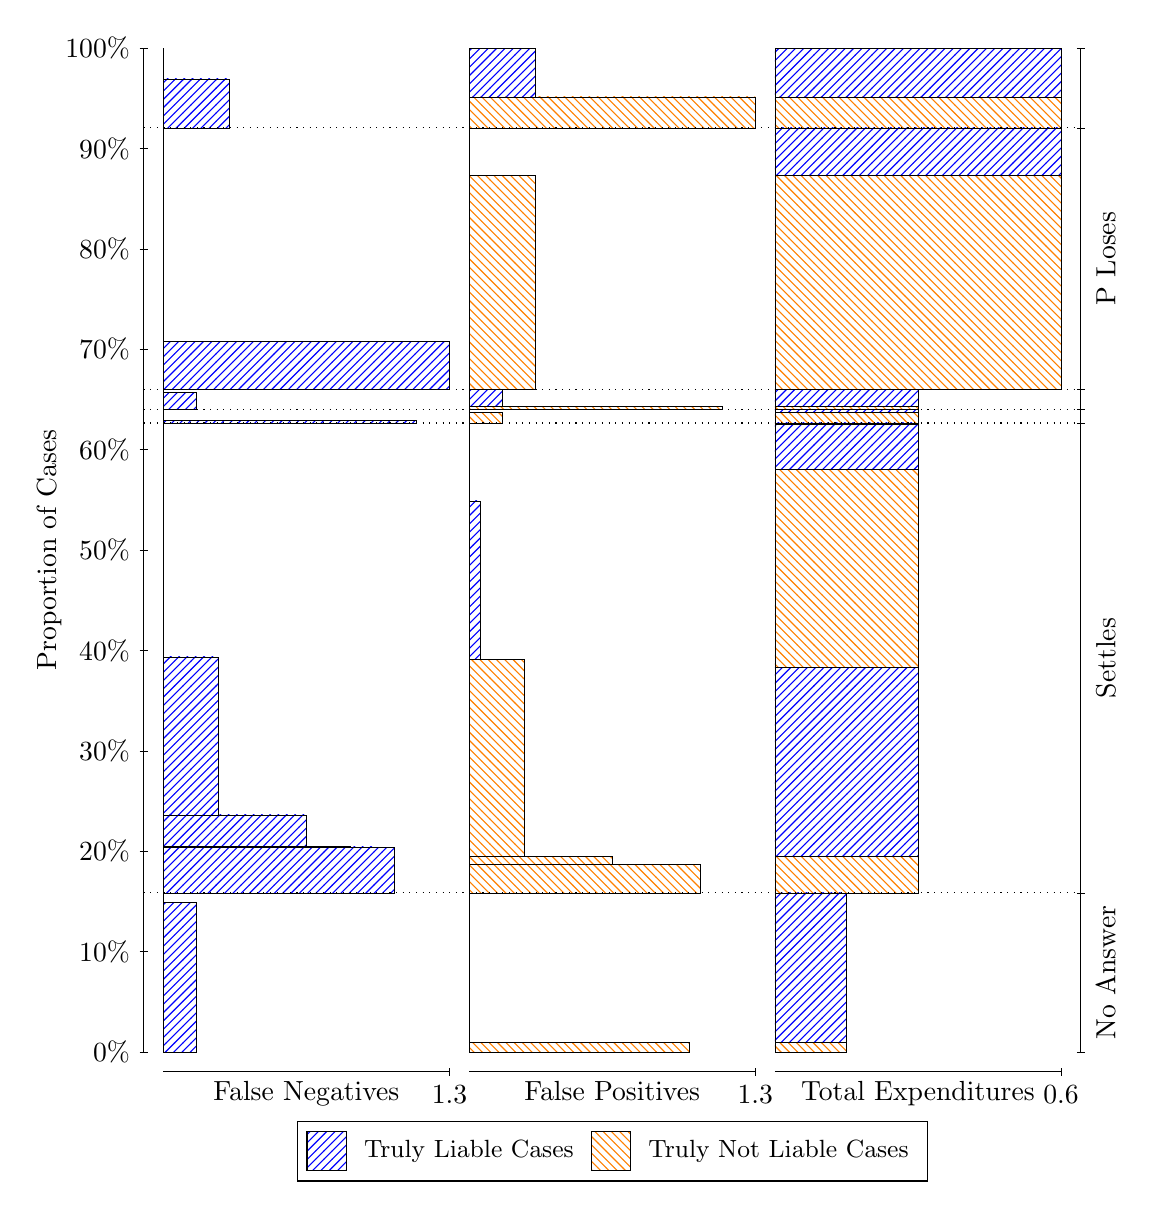
\begin{tikzpicture}
\draw[black, very thin] (1.5,1.75) -- (1.5,14.5);
\node[rotate=90, anchor=center] at (0.3, 8.125) {Proportion of Cases};
\draw[black, very thin] (1.45,1.75) -- (1.55,1.75);
\node[anchor=east] at (1.45, 1.75) {0\%};
\draw[black, very thin] (1.45,3.025) -- (1.55,3.025);
\node[anchor=east] at (1.45, 3.025) {10\%};
\draw[black, very thin] (1.45,4.3) -- (1.55,4.3);
\node[anchor=east] at (1.45, 4.3) {20\%};
\draw[black, very thin] (1.45,5.575) -- (1.55,5.575);
\node[anchor=east] at (1.45, 5.575) {30\%};
\draw[black, very thin] (1.45,6.85) -- (1.55,6.85);
\node[anchor=east] at (1.45, 6.85) {40\%};
\draw[black, very thin] (1.45,8.125) -- (1.55,8.125);
\node[anchor=east] at (1.45, 8.125) {50\%};
\draw[black, very thin] (1.45,9.4) -- (1.55,9.4);
\node[anchor=east] at (1.45, 9.4) {60\%};
\draw[black, very thin] (1.45,10.675) -- (1.55,10.675);
\node[anchor=east] at (1.45, 10.675) {70\%};
\draw[black, very thin] (1.45,11.95) -- (1.55,11.95);
\node[anchor=east] at (1.45, 11.95) {80\%};
\draw[black, very thin] (1.45,13.225) -- (1.55,13.225);
\node[anchor=east] at (1.45, 13.225) {90\%};
\draw[black, very thin] (1.45,14.5) -- (1.55,14.5);
\node[anchor=east] at (1.45, 14.5) {100\%};

\draw[black, very thin] (13.4,1.75) -- (13.4,14.5);
\draw[black, very thin] (13.35,1.75) -- (13.45,1.75);
\node[anchor=west] at (13.35, 1.75) {};
\draw[black, very thin] (13.35,3.77) -- (13.45,3.77);
\node[anchor=west] at (13.35, 3.77) {};
\draw[black, very thin] (13.35,9.738) -- (13.45,9.738);
\node[anchor=west] at (13.35, 9.738) {};
\draw[black, very thin] (13.35,9.9142) -- (13.45,9.9142);
\node[anchor=west] at (13.35, 9.9142) {};
\draw[black, very thin] (13.35,10.168) -- (13.45,10.168);
\node[anchor=west] at (13.35, 10.168) {};
\draw[black, very thin] (13.35,13.486) -- (13.45,13.486);
\node[anchor=west] at (13.35, 13.486) {};
\draw[black, very thin] (13.35,14.5) -- (13.45,14.5);
\node[anchor=west] at (13.35, 14.5) {};

\draw[black, very thin, pattern color=blue, pattern=north east lines] (1.75,1.75) rectangle (2.1692,3.6516);
\draw[black, very thin, pattern color=orange, pattern=north west lines] (1.75,3.6516) rectangle (1.75,3.77);
\draw[black, very thin, pattern color=blue, pattern=north east lines] (1.75,3.77) rectangle (4.6846,4.3495);
\draw[black, very thin, pattern color=blue, pattern=north east lines] (1.75,4.3495) rectangle (4.4051,4.3532);
\draw[black, very thin, pattern color=blue, pattern=north east lines] (1.75,4.3532) rectangle (4.1256,4.3571);
\draw[black, very thin, pattern color=blue, pattern=north east lines] (1.75,4.3571) rectangle (3.8462,4.361);
\draw[black, very thin, pattern color=blue, pattern=north east lines] (1.75,4.361) rectangle (3.5667,4.7596);
\draw[black, very thin, pattern color=blue, pattern=north east lines] (1.75,4.7596) rectangle (2.4487,6.7672);
\draw[black, very thin, pattern color=orange, pattern=north west lines] (1.75,6.7672) rectangle (1.75,9.738);
\draw[black, very thin, pattern color=blue, pattern=north east lines] (1.75,9.738) rectangle (4.9641,9.7752);
\draw[black, very thin, pattern color=orange, pattern=north west lines] (1.75,9.7752) rectangle (1.75,9.9142);
\draw[black, very thin, pattern color=blue, pattern=north east lines] (1.75,9.9142) rectangle (2.1692,10.13);
\draw[black, very thin, pattern color=orange, pattern=north west lines] (1.75,10.13) rectangle (1.75,10.168);
\draw[black, very thin, pattern color=blue, pattern=north east lines] (1.75,10.168) rectangle (5.3833,10.77);
\draw[black, very thin, pattern color=orange, pattern=north west lines] (1.75,10.77) rectangle (1.75,13.486);
\draw[black, very thin, pattern color=blue, pattern=north east lines] (1.75,13.486) rectangle (2.5885,14.108);
\draw[black, very thin, pattern color=orange, pattern=north west lines] (1.75,14.108) rectangle (1.75,14.5);
\draw[black, very thin, pattern color=orange, pattern=north west lines] (5.6333,1.75) rectangle (8.4282,1.8684);
\draw[black, very thin, pattern color=blue, pattern=north east lines] (5.6333,1.8684) rectangle (5.6333,3.77);
\draw[black, very thin, pattern color=orange, pattern=north west lines] (5.6333,3.77) rectangle (8.5679,4.1321);
\draw[black, very thin, pattern color=orange, pattern=north west lines] (5.6333,4.1321) rectangle (7.45,4.2315);
\draw[black, very thin, pattern color=orange, pattern=north west lines] (5.6333,4.2315) rectangle (7.1705,4.2318);
\draw[black, very thin, pattern color=orange, pattern=north west lines] (5.6333,4.2318) rectangle (6.891,4.2321);
\draw[black, very thin, pattern color=orange, pattern=north west lines] (5.6333,4.2321) rectangle (6.6115,4.2323);
\draw[black, very thin, pattern color=orange, pattern=north west lines] (5.6333,4.2323) rectangle (6.3321,6.7407);
\draw[black, very thin, pattern color=blue, pattern=north east lines] (5.6333,6.7407) rectangle (5.7731,8.7484);
\draw[black, very thin, pattern color=blue, pattern=north east lines] (5.6333,8.7484) rectangle (5.6333,9.738);
\draw[black, very thin, pattern color=orange, pattern=north west lines] (5.6333,9.738) rectangle (6.0526,9.877);
\draw[black, very thin, pattern color=blue, pattern=north east lines] (5.6333,9.877) rectangle (5.6333,9.9142);
\draw[black, very thin, pattern color=orange, pattern=north west lines] (5.6333,9.9142) rectangle (8.8474,9.9524);
\draw[black, very thin, pattern color=blue, pattern=north east lines] (5.6333,9.9524) rectangle (6.0526,10.168);
\draw[black, very thin, pattern color=orange, pattern=north west lines] (5.6333,10.168) rectangle (6.4718,12.885);
\draw[black, very thin, pattern color=blue, pattern=north east lines] (5.6333,12.885) rectangle (5.6333,13.486);
\draw[black, very thin, pattern color=orange, pattern=north west lines] (5.6333,13.486) rectangle (9.2667,13.879);
\draw[black, very thin, pattern color=blue, pattern=north east lines] (5.6333,13.879) rectangle (6.4718,14.5);
\draw[black, very thin, pattern color=orange, pattern=north west lines] (9.5167,1.75) rectangle (10.425,1.8684);
\draw[black, very thin, pattern color=blue, pattern=north east lines] (9.5167,1.8684) rectangle (10.425,3.77);
\draw[black, very thin, pattern color=orange, pattern=north west lines] (9.5167,3.77) rectangle (11.333,4.2315);
\draw[black, very thin, pattern color=blue, pattern=north east lines] (9.5167,4.2315) rectangle (11.333,6.6377);
\draw[black, very thin, pattern color=orange, pattern=north west lines] (9.5167,6.6377) rectangle (11.333,9.1461);
\draw[black, very thin, pattern color=blue, pattern=north east lines] (9.5167,9.1461) rectangle (11.333,9.7257);
\draw[black, very thin, pattern color=orange, pattern=north west lines] (9.5167,9.7257) rectangle (11.333,9.7265);
\draw[black, very thin, pattern color=blue, pattern=north east lines] (9.5167,9.7265) rectangle (11.333,9.738);
\draw[black, very thin, pattern color=orange, pattern=north west lines] (9.5167,9.738) rectangle (11.333,9.877);
\draw[black, very thin, pattern color=blue, pattern=north east lines] (9.5167,9.877) rectangle (11.333,9.9142);
\draw[black, very thin, pattern color=orange, pattern=north west lines] (9.5167,9.9142) rectangle (11.333,9.9524);
\draw[black, very thin, pattern color=blue, pattern=north east lines] (9.5167,9.9524) rectangle (11.333,10.168);
\draw[black, very thin, pattern color=orange, pattern=north west lines] (9.5167,10.168) rectangle (13.15,12.885);
\draw[black, very thin, pattern color=blue, pattern=north east lines] (9.5167,12.885) rectangle (13.15,13.486);
\draw[black, very thin, pattern color=orange, pattern=north west lines] (9.5167,13.486) rectangle (13.15,13.879);
\draw[black, very thin, pattern color=blue, pattern=north east lines] (9.5167,13.879) rectangle (13.15,14.5);
\draw[black, dotted] (1.5,3.77) -- (13.4,3.77);
\draw[black, dotted] (1.5,9.738) -- (13.4,9.738);
\draw[black, dotted] (1.5,9.9142) -- (13.4,9.9142);
\draw[black, dotted] (1.5,10.168) -- (13.4,10.168);
\draw[black, dotted] (1.5,13.486) -- (13.4,13.486);
\draw[black, very thin] (1.75,1.5) -- (5.3833,1.5);
\node[anchor=north] at (3.5667, 1.5) {False Negatives};
\draw[black, very thin] (5.3833,1.45) -- (5.3833,1.55);
\node[anchor=north] at (5.3833, 1.45) {1.3};

\draw[black, very thin] (5.6333,1.5) -- (9.2667,1.5);
\node[anchor=north] at (7.45, 1.5) {False Positives};
\draw[black, very thin] (9.2667,1.45) -- (9.2667,1.55);
\node[anchor=north] at (9.2667, 1.45) {1.3};

\draw[black, very thin] (9.5167,1.5) -- (13.15,1.5);
\node[anchor=north] at (11.333, 1.5) {Total Expenditures};
\draw[black, very thin] (13.15,1.45) -- (13.15,1.55);
\node[anchor=north] at (13.15, 1.45) {0.6};

\node[black, centered, rotate=90] at (13.72, 2.76) {No Answer};
\node[black, centered, rotate=90] at (13.72, 6.754) {Settles};


\node[black, centered, rotate=90] at (13.72, 11.827) {P Loses};


\draw (7.449999999999999,1.5) node[draw=none] (baseCoordinate) {};
\begin{scope}[align=center]
        \matrix[scale=0.5, draw=black, below=0.5cm of baseCoordinate, nodes={draw}, column sep=0.1cm]{
            \node[rectangle, draw, minimum width=0.5cm, minimum height=0.5cm, pattern=north east lines, pattern color=blue] {}; &
            \node[draw=none, font=\small] (B) {Truly Liable Cases}; &
            \node[rectangle, draw, minimum width=0.5cm, minimum height=0.5cm, pattern=north west lines, pattern color=orange] {}; &
            \node[draw=none, font=\small] (B) {Truly Not Liable Cases}; \\
            };
\end{scope}

\end{tikzpicture}
\end{document}